\documentclass[11pt]{article}

\usepackage{fullpage}
\usepackage{url}
\usepackage{todonotes}
\usepackage{amsmath}
\usepackage{amsthm}
\usepackage{amsfonts}
\usepackage{amssymb}
\usepackage[utf8]{inputenc}
\usepackage{soul}
\usepackage{multicol}
\usepackage[numbers]{natbib}
\usepackage[ruled, vlined, linesnumbered]{algorithm2e}
\usepackage{placeins}
\usepackage{hyperref}

% Theorem and Math macros borrowed from 
% CS Professor Matt Anderson
% ------- Theorem and related environments --------
\newtheorem{theorem}{Theorem}
\newtheorem{conjecture}{Conjecture}
\newtheorem{proposition}{Proposition}
\newtheorem{claim}{Claim}
\newtheorem{lemma}{Lemma}
\newtheorem{corollary}{Corollary}
\newtheorem{definition}{Definition} 
\newtheorem{problem}{Problem}
\newtheorem{observation}{Observation}
\newtheorem{fact}{Fact}

\newcommand{\NN}{\mathcal{N}} % Natural Numbers
\newcommand{\RR}{\mathcal{R}} % Real Numbers
\newcommand{\ZZ}{\mathcal{Z}} % Integers
\newcommand{\QQ}{\mathcal{Q}} % Rational Numbers

\newcommand{\set}[1]{\ensuremath{\{{#1}\}}} % Set
\newcommand{\bigset}[1]{\ensuremath{\left\{{#1}\right\}}}
\newcommand{\condset}[2]{\ensuremath{\set{{#1}\;|\;{#2}}}} % Conditional set
\newcommand{\nin}{\not\in}
\newcommand{\cross}{\times} % Cartesian product
\newcommand{\ssn}{\subsetneq} % Proper subset
\newcommand{\sse}{\subseteq} % Subset

\DontPrintSemicolon
\newcommand{\spa}{\rightsquigarrow}
\newcommand{\td}{\todo[inline]}

\begin{document}

\title{Heuristic Algorithms for Bike Route Generation}
\author{Aidan Pieper}
\maketitle

\td{Write Abstract!}
\section{Introduction}
Cycling is a popular and diverse activity enjoyed by millions of people all over the world. To some, cycling is a means of commuting to work while to others it is a recreational sport. Furthermore, the quality of cycling-specific infrastructure is varied across the globe. In countries like Belgium and the Netherlands where cycling is a popular recreational sport, there are vast networks of bicycle-friendly secondary roads \cite{souffriau2011planning}. However, many places do not have this same level of cycling infrastructure so bike riders must share highways with other road vehicles.


When determining routes to bike, recreational cyclists often weigh many different factors such as route distance, elevation gain (i.e. hills), maximum percent gradient (i.e. road steepness), and how pleasant a road is to travel by bike. Designing a route that fits all user-specified criteria is often a very difficult or impossible task.  Moreover, there are no set criteria which determine a ``preferable" cycling route. The desirability of a given cycling route is very much based on the rider's personal preferences, goals, and fitness. This research explores different algorithms to generate cycling routes for recreational road cyclists.


Most bike rides begin and end in the same location. Using this assumption, this research focuses specifically on generating preferable \emph{circular} cycling routes. For example, a recreational cyclist may want a 15-mile route with minimal traffic which starts and ends at their home.
    

\subsection{Motivations}
Traditional route planning problems focus mainly on finding the shortest path in a graph (i.e. road network) optimizing for either distance or time. Currently, there exists numerous route planning tools (e.g. \href{https://www.strava.com/routes/new}{Strava.com}, \href{https://www.mapmyride.com}{mapmyride.com}, and \href{https://ridewithgps.com}{ridewithgps.com}) which allow users to add points on a map and generate a route between such destinations.

However, route planning for recreational cyclists poses a fundamentally different problem than traditional route planning problems because the shortest route is not necessarily the 	preferable cycling route. Recreational cyclists generally prefer longer, more scenic, and less trafficked routes as the goal of the activity is recreation not transportation. Since recreational cyclists include many factors when determining a ride, a cycling route planning problem should optimize for more than just distance or time.   

\subsection{Related work} \label{relatedwork}
In previous literature, the problem of planning preferable cycling routes can be modeled as an instance of the Arc Orienteering Problem (AOP), a variant of the Orienteering Problem (OP) \cite{souffriau2011planning}. First introduced in 1987 by \citeauthor{golden1987orienteering}, the classical OP is a combination of node selection and determining shortest paths between nodes in a graph \cite{golden1987orienteering}. In other words, the OP is a hybrid between two classical combinatorial problems, the Knapsack Problem and the Traveling Salesman Problem (The OP may sometimes be referred to as the \emph{Selective} Traveling Salesman Problem \cite{laporte1990selective}). In the classical OP, each node in the graph is assigned a non-negative score and a non-negative cost. Given a starting node, a destination node, and some maximum budget, the objective of the problem is to determine a path which starts at the starting node, visits some subset of the graph nodes, and ends at the destination node \cite{gunawan2016orienteering}. In addition, the path must both maximize the total collected score (accrued from visiting a node) and keep the total collected cost under the specified budget.

The AOP is the arc variant of the OP. In the AOP, each arc (i.e. graph edge) is given a score and a cost. The goal of the AOP is produce a path which maximizes the collected score by \emph{visiting arcs} while keeping the cost within the given budget. The fundamental difference between these two problems is that one visits nodes of the graph (OP) while the other visit edges (AOP). In other words, one problem associates profit with the nodes and the other associates profit with arcs. For example, Figure \ref{fig:aop-example} shows an undirected AOP instance where $S$ is the start node, $D$ is the destination node, the budget is 10, and every edge is labeled (score, cost). The shortest path is $S \rightarrow (10,3) \rightarrow (5,5) \rightarrow D$ which has a cost of 8 and a score of 15. However, for the specified budget, $S \rightarrow (20,1) \rightarrow (3,2) \rightarrow (2,2) \rightarrow (5,5) \rightarrow D$ is the optimal solution with a score of 30 and a cost of 10. Note that the optimal solution is clearly not the shortest path but rather the path with the maximal score constrained by the cost budget.

Previous research has shown that both the OP and the AOP are NP-Hard problems for directed and undirected graphs. Therefore, no algorithms are known to exist to \emph{optimally} solve the AOP or OP in polynomial time. While there is considerable research into the OP and its variants, there is less research into the AOP. \citeauthor{gunawan2016orienteering} provide an exhaustive survey of the OP and its variants, but the AOP is clearly over shadowed by other OP variants in the literature \cite{gunawan2016orienteering}.

\begin{figure}[h]
\begin{center}
    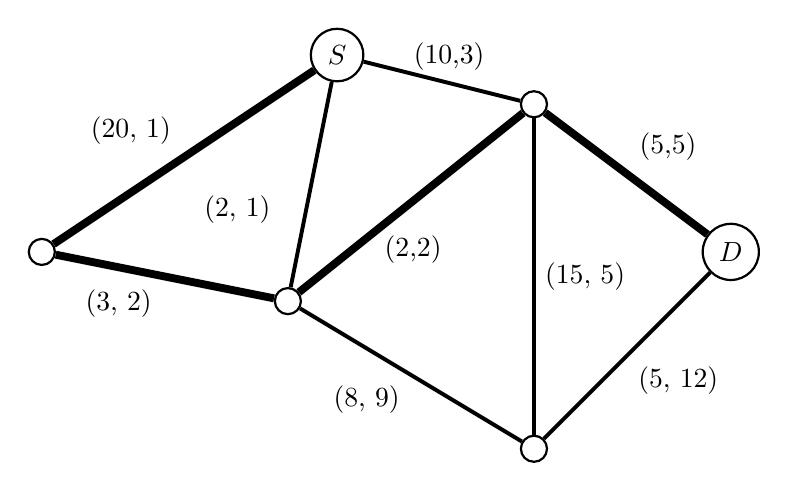
\begin{tikzpicture}[auto,x=1.25cm, y=1.25cm,line width=0.5mm]
    
        \begin{scope}[every node/.style={circle,thick,draw}]
        \node(1) at (0,0) {$S$};
        \node(2) at (2, -0.5) {};
        \node(3) at (4, -2) {$D$};
        \node(4) at (2, -4) {};
        \node(5) at (-0.5, -2.5) {};
        \node(6) at (-3, -2) {};
        \end{scope}
        
        \draw (1) -- node[xshift=-0.5cm] {(10,3)} (2);
        \draw[line width=1mm]  (2) -- node {(5,5)} (3);
        \draw (3) -- node {(5, 12)} (4);
        \draw (2) -- node {(15, 5)} (4);
        \draw[line width=1mm] (2) -- node[yshift=-0.25cm, xshift=-0.5cm] {(2,2)}(5);
        \draw (4) -- node {(8, 9)}(5);
        \draw[line width=1mm] (5) -- node {(3, 2)} (6);
        \draw[line width=1mm] (6) -- node[] {(20, 1)} (1);
        \draw (1) -- node [xshift=-1.5cm]{(2, 1)} (5);
    
    \end{tikzpicture}
\end{center}
\caption{Undirected AOP instance with start node $S$ and destination $D$. Arc label is (score, cost). Bold path is optimal for a budget of 10 (score = 30, cost = 10). Note that the bold path is not the shortest path.\label{fig:aop-example}}
\end{figure}

 
\citeauthor{gavalas2015approximation} show approximation algorithms for the AOP in both directed and undirected graphs. A polylogarithmic approximation algorithm is given for directed graphs while a $(6 + \epsilon + o(1))$-approximation algorithm is given for undirected graphs \cite{gavalas2015approximation}. Moreover, they show a reduction from the AOP to the OP. Using an existing OP approximation algorithm by \citeauthor{nagarajan2011directed}, this reduction yields a $O(\frac{log^2m}{loglogm})$-approximation algorithm for solving the AOP in directed graphs where $m$ is the number of edges \cite{gavalas2015approximation}.

Both \citeauthor{souffriau2011planning} and \citeauthor{verbeeck2014extension} study the AOP in the context of cycle trip planning. \citeauthor{souffriau2011planning} provide an integer programming mathematical model for the AOP and a heuristic algorithm for solving AOP instances to near optimality in a few seconds. To evaluate performance of their algorithm, the authors test their algorithm against a road network of bike-friendly roads in East Flanders \cite{souffriau2011planning}. The East Flanders' bicycle road network covers 5 regions and is comprised of 989 nodes with 2963 arcs for a total of 3585 km (2227 mi) of road. This model for the AOP, tailored towards recreational cycling routes, requires that each node and edge is visited at most once by the solution path and prevents sub-tours. \citeauthor{souffriau2011planning} present an algorithm based on a greedy randomized adaptive search procedure method \cite{souffriau2011planning}.

On the other hand, \citeauthor{verbeeck2014extension} consider the cycle trip planning problem in a directed graph where the goal is to maximize the total collected score which represents the attractiveness of the travelled arcs. In this model, the preferred length of the route is replaced with an upper and lower bound of the total trip distance. Unlike, \citeauthor{souffriau2011planning}, this model allows the route to visit the same vertex multiple times but visiting the same arc twice is not allowed. A two-way road can be travelled exactly once in each direction since it is modeled by two separate edges in the directed graph. The authors propose two heuristic algorithms for solving cycle trip planning instances; A branch-and-cut algorithm and an iterated local search algorithm \cite{verbeeck2014extension}. Both algorithms were evaluated by running them on the East Flanders road network dataset provided by \citeauthor{souffriau2011planning}

Similarly, research by \citeauthor{bergman2015optimization} defines the ``Circular Cycle Tour Problem" as a cycle trip planning problem where the start and end location are the same. Like other cycle trip planning problems, they model it as an instance of the AOP. \citeauthor{bergman2015optimization} use a popularity weighted road network graph using road popularity data from smartphone fitness tracking application \href{http://www.sports-tracker.com/}{sports-tracker.com} (i.e, the most popular roads have high positive scores) \cite{bergman2015optimization}. They present a heuristic algorithm that starts with initial random cyclic routes and iteratively improves them to find a locally optimal route. As well as maximizing the popularity of travelled roads, the generated routes avoid traversing the same road twice, avoid sub-loops, cover a wide area, and are close to the target length set by the user. In their research, the assumption that \citeauthor{bergman2015optimization} make is that the most popular roads among other athletes are the most preferable to bike on.

\subsection{Modeling Preferability of Cycling Routes} \label{routefactors}
As mentioned previously, recreational cyclists consider many factors when designing a preferable cycling route. The following is a non-exhaustive list of such factors:

\begin{multicols}{2}
\begin{itemize}
    \item Route distance
    \item Route elevation gain
    \item Time
    \item Maximum percent gradient
    \item Amount of traffic
    \item Number of intersections
    \item Good cellular service
    \item Easy parking at start
    \item Availability of restrooms
    \item Availability of rest stops and food
    \item Scenery
    \item Proximity to bike shops
    \item Proximity to mass transit
    \item Limited uphill at end of ride
\end{itemize}    
\end{multicols}

Many of these factors can be modeled nearly identically. For example, distance, elevation gain, and time are all calculated by the sum of those weights over all roads in the route. On the other hand, maximum percent gradient can be seen as a ``boolean criterion." That is, a road's steepness is either under the maximum percent gradient or over, in which case the road does not satisfy this criterion. If these boolean criteria must be avoided, a simple option is to initially remove or ``prune" all roads from the graph which do not meet these criteria.

In previous research, the cost of a particular arc is usually the distance of the  road and the score is some measure of the preferability of the road (e.g. popularity). Since the AOP requires a single value for the cost and score of each arc, computing costs and scores as linear combinations of different variables is a one way to model multiple factors. For example, a particular road's cost might be a combination of its distance, its elevation gain, and how much traffic is on the road. This allows one to give certain factors more importance by weighting them more heavily in the linear combination. Furthermore, one might want to avoid certain boolean criteria instead of outlawing them entirely. For instance, one could give the presence of a dirt road a small weight in the cost of a road which means dirt roads will have slightly higher costs.

While multiple route factors are important to recreational cyclists, the main goal of this research is not to model preferability of roads. Hence, we will assume that we have the necessary data to appropriately score roads for recreational cyclists. In other words, the focus of this research is on the route planning algorithm, not creating the graph (with the associated scores and costs) which represents the AOP instance.


\subsection{Research Question}
The end goal of this research is to produce an algorithm that generates good circular cycling routes whose distances are within the specified budget. As mentioned in Section \ref{relatedwork}, existing cycle trip planning algorithms model this problem as an instance of the AOP. This research follows the existing literature and focuses on implementing and improving existing AOP algorithms for cycle route planning. 

Since road networks can be quite large and because the AOP is NP-Hard, searching for the optimal route may take an unacceptable amount of time. Because I care more about finding a good route than finding the best possible route, I will give up optimality for speed. However, even AOP approximation algorithms are too slow for applications where a fast response time (on the order of milliseconds) is required \cite{lu2015arc}. Therefore, I will focus on heuristic algorithms for route generation. Both \citeauthor{verbeeck2014extension} and \citeauthor{lu2015arc} propose heuristic algorithms which follow the Iterated Local Search (ILS) framework. This framework, and their respective algorithms are the focus of the following sections. More specifically, in this research I will analyze and improve existing ILS algorithms. Thus, the research question is as follows:

\begin{quote}
    To what extent can ILS algorithms be improved to generate better bike routes?
\end{quote}

In the following sections I will refer to the the algorithm proposed by \citeauthor{verbeeck2014extension} as the \emph{VVA algorithm}. Furthermore, I will refer to the algorithm proposed by \citeauthor{lu2015arc} as the \emph{Lu-Shahabi algorithm}.


\section{Methods}

\subsection{Iterated Local Search}
Iterated Local Search (ILS) is a framework for solving optimization problems using heuristic search algorithms. A heuristic is a technique used to solve a problem quickly when exact or approximation methods are too slow. Heuristic algorithms can be thought of as ``shortcuts" in that they trade optimality and completeness for speed. Heuristics are often used in search algorithms to  determine which branch of the search to take but are not guaranteed to produce the best solution. A heuristic algorithm is commonly referred to as a heuristic.

Local search (LS) is a heuristic method for solving optimization problems. LS starts with a candidate solution and moves to a ``neighbor" solution which is better than the current solution as defined by an objective function (a function which scores solutions in the search space) \cite{gendreau2010handbook}. LS can get stuck in local optima which are points in the search space that are better than all neighbors but are not the best possible solution.

ILS can be thought of as a modification of LS to stop it from getting trapped in local optima. Instead of repeating random trials of the heuristic algorithm, ILS builds a sequence of locally optimal solutions generated by the heuristic which is more likely to lead to a better overall solution \cite{gendreau2010handbook}. This is done by first generating an initial solution using the search heuristic, perturbing the current solution (or changing the solution), and applying the search heuristic again on the modified solution. The perturbation and local search steps are then repeated until some condition, usually time, is met.
The following pseudocode outlines the ILS framework:

%
% Iterated Local Search definition
%
\begin{algorithm}[!h]
\caption{ILS($t$, $localsearch$, $score$)}
\KwData{$t$: a time, $localsearch$: a heuristic search function, $score$: an objective function.}
\KwResult{A solution of the $localsearch$ function.}
S $\gets$ $localsearch$(empty solution)\;
\While{$t$ seconds have not elapsed}{
    $S^* \gets$ perturb $S$\;
    $S' \gets localsearch(S^*)$\;
    \If{$score(S') > score(S)$}{
        $S \gets S'$\;
    }
}
\KwRet{S}
\end{algorithm}

Despite its simplicity, ILS can be challenging to implement efficiently because many implementation choices are left to the developer. For example, an efficient ILS implementation requires a certain level of domain specific knowledge. The main issue with ILS is that the algorithm may get ``trapped" in a local maximum over many iterations. Therefore, the modification (perturbation) step must modify the search solution enough to make progress but not too much that the search is effectively starting with a different ``random" solution upon each iteration. 

% TODO(Aidan) draw picture of ils peaks and troughs


\subsection{VVA Algorithm}
%\td{The graph $G$ is never passed in anywhere in the pseudocode??}
The local search algorithm used by \citeauthor{verbeeck2014extension} is a modified version of depth first search (Algorithm \ref{alg:dfs}). It is implemented as a recursive function which used to to find a path between two disconnected nodes in the bike route. The algorithm works by choosing arcs which increase the score while not violating the maximum distance constraint of the route. The algorithm starts at the start node $s$ and iterates over all possible outgoing edges one at a time traversing the graph in a depth first fashion (Lines \ref{alg:dfs:for}-\ref{alg:dfs:endfor}). The algorithm is allowed to ``take" an outgoing edge and add it to the current route as long as it has not been traversed before (already in the route) and the shortest path from the end of the traversed arc to the destination is less than the remaining distance after taking the arc (Line \ref{alg:dfs:feasability}). In other words, it must be \emph{feasible} to get from the end of this arc to the desired destination after traversing the arc.

If the end of the arc chosen is the destination and the total accrued score is above the $minProfit$ threshold, the algorithm has a valid path in $route$ and returns true (Line \ref{alg:dfs:end}). Otherwise, the algorithm has not found a path to the destination and recurses. After adding an arc to the solution, the algorithm needs to find a path from the end of the arc just inserted to the destination (Line \ref{alg:dfs:recurse}). In addition, adding an arc to the solution decreases the remaining distance budget left and the max depth by one. The $maxDepth$ parameter is used to restrict the depth of the search and reduce the search space (Line \ref{alg:dfs:depth}).

\begin{algorithm}[!h]
    \caption{DFS($route$, $s$, $d$, $dist$, $minProfit$, $maxDepth$)\label{alg:dfs}}
    \KwData{$route$: a temporary solution, $s$: the start node of the path, $d$: the end node of the path, $dist$: the maximum cost of the route, $minProfit$: the minimum score of the route, $maxDepth$: the maximum number of edges allowed in the solution, $shortestPath(v_1, v_2)$: a function which returns the shortest distance between two nodes of the graph, and $edges(v_1)$: a function which returns all edges of a node. 
        }
    \KwResult{A boolean which denotes whether a path was found. If true, the solution is contained inside of $route$.}
    \If{$maxDepth < 0$}{\label{alg:dfs:depth}
        \KwRet{false}\;
    }
    \For{$arc \in edges(s)$}{ \label{alg:dfs:for}
        \If{$arc \nin route$ and $arc.cost + shortestPath(arc.end, d) < dist$}{\label{alg:dfs:feasability}
            Add $arc$ to $route$\;
            \uIf{$arc.end = d$ and $route.score > minProfit$}{\label{alg:dfs:end}
                \KwRet{true}\;
            } \ElseIf{DFS(route, arc.end, d, dist - arc.cost, minProfit, maxDepth - 1)}{\label{alg:dfs:recurse}
                \KwRet{true}\;
            }
            Remove $arc$ from $route$\;
        }\label{alg:dfs:endfor}
    }
\KwRet{false}\;
\end{algorithm} 

Using this DFS algorithm as the local search heuristic \citeauthor{verbeeck2014extension}, apply the ILS framework to create a bike route planning algorithm. Algorithm \ref{alg:ils-ver} first generates an initial route using the DFS heuristic and stores the path in the variable $route$ (Line \ref{alg:ilsv:init}). The ILS perturbs the solution by removing a path segment from the solution and invoking the DFS procedure to find a new solution (Lines \ref{alg:ilsv:perturb}-\ref{alg:ilsv:improve}). In the perturbation phase, the algorithm removes $R$ consecutive arcs starting at the arc at position $A$ in solution $route$. If a new path is found after removing a path segment from the solution, then the new path is merged into the current solution (Line \ref{alg:ilsv:merge}). If no new path can be found, then there is no improvement so $A$ and $R$ are both incremented by 1 (Line \ref{alg:ilsv:increment}).

%
% VVA ILS Algorithm
%
\begin{algorithm}[!h ]
    \caption{ILS-VVA($s$, $d$, $dist$, $maxDepth$, $t$) \label{alg:ils-ver}}
    \KwData{$s$: the start node of the path, $d$: the end node of the path, $dist$: the maximum distance of the path, $maxDepth$: the maximum depth allowed in the DFS, and $t$: a time.}
    \KwResult{a path.}
    
    $route \gets$ empty route\;
    \If{not DFS(route, s, d, dist, 0, maxDepth)}{\label{alg:ilsv:init}
        $route \gets$ empty route\;
    }
    $A \gets 1$, $R \gets 1$\;
    
    \While{$t$ seconds have not elapsed}{
        $temp \gets$ copy of $route$\;
        \If{$R > temp.length$}{
            $R \gets 1$\;
        }
        
        \If{$A + R > temp.length -1$}{
            $R \gets temp.length - 1 - A$\;
        }
        
    
        Remove $R$ arcs from $temp$ starting at arc at index $A$\; \label{alg:ilsv:perturb}
        $minScore \gets$ sum of scores of removed arcs from $temp$\;
        $s^* \gets$ starting node of first arc removed\;
        $d^* \gets$ ending node of last arc removed\;
        $new \gets$ empty route\;
        
        \If{DFS(new, $s^*$, $d^*$, dist - temp.dist, minScore, maxDepth)}{\label{alg:ilsv:improve}
            Merge $new$ into $temp$ at index $A$\; \label{alg:ilsv:merge}
            $route \gets temp$\;
            $A \gets 1$, $R \gets 1$\;
        } \Else {
            $A \gets A + 1$, $R \gets R + 1$\; \label{alg:ilsv:increment}
        }
    
    }
    
    \KwRet{route}        
\end{algorithm}

\subsection{Lu-Shahabi Algorithm}
The main drawback of the VVA algorithm is that the ILS has slow iteration because it is performing DFS on every iteration. Since the algorithm assumes all pairs shortest-path pre-computated, the feasibility checking used by the search is $O(degree^{maxDepth})$ where $degree$ is the average degree of nodes in the road network and $maxDepth$ is the maximum depth allowed in the DFS.

At a high level, the series of algorithms proposed by \citeauthor{lu2015arc} utilize ILS but aim to restrict the search space by using spatial indices to prune arcs from the search. Instead of relying on pre-computed shortest paths, the Lu-Shahabi algorithms use online shortest path computations but do less feasibility checking due to the spatial restrictions (See Section \ref{sec:pruning} for more information). In addition, \citeauthor{lu2015arc} propose two new heuristics which are used to determine how to add and remove arcs from the solution such that the overall score improves.
\subsubsection{Problem Statement}
Unlike \citeauthor{verbeeck2014extension}, \citeauthor{lu2015arc} define their solution route in terms of ``attractive arcs" which are arcs with a positive score (i.e. $arc.score > 0$). A path from node $v_1$ to $v_2$ is a series of attractive arcs $(a_1, a_2, \ldots, a_n)$ which starts with $a_1$, ends with $a_n$ and is denoted by, $(v_1 \spa a_1 \spa a_2 \spa \ldots \spa a_n \spa v_2)$. The symbol $\spa$ denotes the shortest path in the graph between two nodes or arcs. The path between two adjacent attractive arcs ($a_i \spa  a_{i+1}$) is known as the ``blank path segment" and is the shortest path from the end vertex of $a_i$ to the start vertex of $a_{i+1}$. These vertices are respectively denoted $l_i.start$ and $l_i.end$. Given an attractive arc $a_i$ from a solution path, $a_i.pre$ refers to the previous attractive arc ($a_{i-1}$) and $a_i.post$ refers to the next attractive arc in the path ($a_{i+1}$). The total cost of a path is the sum of all costs of all the arcs in the path, including the arcs in the blank path segments. The score of a path is defined similarly.

\subsubsection{Search Heuristics}


 Since these algorithms utilize the ILS framework (like \citeauthor{verbeeck2014extension}), the main issues are as follows:
\begin{enumerate}
    \item How should arcs be removed from the solution so that solution's score improves?
    \item How should arcs be selected to update the solution so that the solution's score improves?
\end{enumerate}
In order to address these questions, \citeauthor{lu2015arc} apply two criteria onto a set of arcs. That is, every arc $a$ in the solution $S$ is associated with a set of candidate arcs. 
%
% Definition of Candidate Arc Set
%
\begin{definition}[\cite{lu2015arc}]
    Let $a \in S$ be an arc in the solution $S$ whose distance budget is $B$. Then the Candidate Arc Set (CAS) of $a$, denoted by $a.CAS$ is the set of arcs who have a positive score and can feasibly update (replace) $a$ in $S$, i.e. $\forall a_c \in a.CAS, a_c.score > 0$ and $(a.pre \spa a_c \spa a.post).cost < B - S.cost + (a.pre \spa a \spa a.post)$.
\end{definition}

\citeauthor{lu2015arc} show that candidate arc sets have the following inherited property. This allows the search space to be reduced when computing some candidate arc sets since the parent sets can be restricted.
\begin{lemma}[\cite{lu2015arc}] Let $a$ be an arc. Given $a.CAS$, $\forall a_c \in a.CAS, a_c.CAS \sse a.CAS$.
\end{lemma}

In order to determine which arcs to choose to improve the solution, they propose a criteria called ``QualityRatio" (Algorithm \ref{alg:ils-lu-qr}) which is defined for an arc $a_c$ from the candidate arc set $a.CAS$ of a solution arc $a$. The intuition is that arcs with higher value and lower cost will be more likely to improve the solution. This criteria will be used to pick arcs to add to the solution.

%
% Quality Ratio algorithm
%
\begin{algorithm}[!h]
    \caption{QualityRatio($a.pre$, $a.post$, $a_c$) \label{alg:ils-lu-qr}}
    \KwData{$a_c$: arc from candidate arc set, $a.pre$: previous arc in solution, $a.post$: next arc in solution.}
    \KwResult{a number.}
    $score \gets (a.pre \spa a_c \spa a.post).score$\;
    $cost \gets (a.pre \spa a_c \spa a.post).cost$\;
    \KwRet{$score / cost$}        
\end{algorithm}

In order to determine which arcs to remove from the solution, they propose a criteria called ``ImprovePotential" (Algorithm \ref{alg:ils-lu-ip}). The intuition is that solution arcs with lower scores and more valuable nearby arcs are more likely to improve the solution. This criteria will be used to pick arcs from the solution to be removed.

%
% Improve Potential algorithm
%
\begin{algorithm}[!h]
    \caption{ImprovePotential($a$) \label{alg:ils-lu-ip}}
    \KwData{$a$: a solution arc}
    \KwResult{a number.}
    $score \gets 0$\;
    $maxDist \gets 0$\;
    $dist \gets (a.pre \spa a \spa a.post).cost$\;
    \For{$e \in a.CAS$}{
        $score \gets score + (e.score - a.score)$\;
        $maxDist \gets max(maxDist, (a.pre \spa e \spa a.post).cost)$\;
    }
    \KwRet{$score / (maxDist - dist)$}       
\end{algorithm}

%
% Compute Candidate Arc Set algorithm
%
\begin{algorithm}[!h]
    \caption{computeCAS($G$, $A$, $v_1$, $v_2$, $dist$) \label{alg:ils-lu-compcas}}
    \KwData{$G$: the road network graph, $A$: a candidate arc set, $v_1$: start node, $v_2$: destination node, $dist$: allowable budget.}
    \KwResult{A set of candidate arcs.} 
    $CAS \gets \text{empty set}$\;
    \If{$A$ is empty}{ \label{alg:ils-lu-compcas-if}
    $A \gets$ all arcs from $G$\; \label{alg:ils-lu-compcas-ifend}
    }
    \For{$a \in A$}{\label{alg:ils-lu-compcas-for}
        \If(\tcp*[h]{Feasibility checking}){$a.score > 0$ and $(v_1 \spa a \spa v_2).cost \leq dist)$}{
            $a.qr = QualityRatio(v_1, v_2, a)$\; \label{alg:ils-lu-compcas-qr}
            add $a$ to CAS\; \label{alg:ils-lu-compcas-add}
        }
    }
    \KwRet{CAS}
\end{algorithm}


\subsubsection{Generating Candidate Arc Sets}

Algorithm \ref{alg:ils-lu-compcas} performs the feasibility checking to generate a set of candidate arcs which can be used to connect the start node $v_1$ to the destination node $v_2$. The algorithm takes in a set of possible arcs, iterates over each one, and adds the arc to the current CAS only if its score is positive and the distance of the path from $v_1$ to $a$ to $v_2$ is within the specified budget (Lines \ref{alg:ils-lu-compcas-for}-\ref{alg:ils-lu-compcas-add}). In addition, the quality ratio (Algorithm \ref{alg:ils-lu-qr}) is calculated for the specified arc in the CAS (Line \ref{alg:ils-lu-compcas-qr}). If the CAS, $A$, passed into the algorithm is non-empty, then it can use the ``CAS inherit" property and filter out arcs whose paths are within the new specified budget. If the CAS passed in is non-empty, then the algorithm will iterate over all arcs in the graph to find the ones which can be feasibly inserted (Lines \ref{alg:ils-lu-compcas-if}-\ref{alg:ils-lu-compcas-ifend}).


%
% Update Candidate Arc Set algorithm
%
\begin{algorithm}[!h]
    \caption{updateCAS($A$, $a$, $v_1$, $v_2$, $newDist$, $oldDist$) \label{alg:ils-lu-updatecas}}
    \KwData{$A$: set of all arcs in the graph, $a$: arc whose CAS needs to be updated, $v_1$: node in current path before $a$, $v_2:$ node in current path after $a$, }
    \KwResult{An updated set of candidate arcs}
    $CAS \gets a.CAS$\;
    \If(\tcp*[h]{Restrict CAS using inherit property}){$newDist < oldDist$}{\label{alg:ils-lu-updatecas-less}
        \For{$e \in a.CAS$}{
            \If{$(v_1 \spa e \spa v_2).cost > newDist$}{
                remove $e$ from $CAS$\; \label{alg:ils-lu-updatecas-lessend}
            }
        }
    } \ElseIf(\tcp*[h]{Expand CAS by checking all edges from graph}) {$newDist > oldDist$}{ \label{alg:ils-lu-updatecas-more}
        \For{$e \in A$}{
            \If{$e \nin CAS$ and $e.score > 0$ and $(v_1 \spa e \spa v_2).cost \leq newDist$}{
                add $e$ to $CAS$\; \label{alg:ils-lu-updatecas-moreend}
            }
        }
    }
    \KwRet{CAS}
\end{algorithm}

Algorithm \ref{alg:ils-lu-updatecas}'s job is to update the CAS for a particular arc $a$. If arcs are added to the current solution, then its distance changes as well as the remaining budget. For the new arcs added, computing the respective CASs using Algorithm \ref{alg:ils-lu-compcas} suffices. However, the previous arcs in the solution need to have their CASs changed since the remaining distance (budget) is now different. Algorithm \ref{alg:ils-lu-updatecas} takes in two budget values, $newDist$ and $oldDist$. If the new budget is smaller than the old budget, there may be some arcs in our CAS whose paths are too long for the new budget. Therefore, the algorithm employs CAS inheritance and restricts the current CAS by removing the arcs which can no longer be feasibly inserted with the new budget (Lines \ref{alg:ils-lu-updatecas-less}-\ref{alg:ils-lu-updatecas-lessend}). If the new budget is larger than our old budget, then the algorithm must expand the CAS by checking the feasibility of all arcs in the graph (Lines \ref{alg:ils-lu-updatecas-more}-\ref{alg:ils-lu-updatecas-moreend}).


\subsubsection{ILS Implementation}
Algorithm \ref{alg:ils-lu-genpath} is the local search heuristic used by the ILS (Algorithm \ref{alg:ils-lu}). Its goal is to produce a path which connects the start vertex $s$ with the destination vertex $d$ whose total cost is within the budget $dist$ and total score is greater than $minProfit$. The algorithm builds the path by choosing candidate arcs from the CAS $A$.

Algorithm \ref{alg:ils-lu-genpath} first instantiates a fake arc starting and ending at the specified endpoints with a cost and score of 0 (Line \ref{alg:ils-lu-genpath-fake}). This fake arc is used to instantiate the solution to return, $route$ (Line \ref{alg:ils-lu-genpath-init}). It then obtains a set of arcs to insert by filtering the CAS $A$ by choosing arcs whose quality ratio is higher than the average (Line \ref{alg:ils-lu-genpath-arcs}). While there are still possible arcs left to insert and the path has budget left, arcs are continuously removed from the CAS and inserted into the current solution $route$ (Lines \ref{alg:ils-lu-genpath-while}-\ref{alg:ils-lu-genpath-endwhile}). The algorithm inserts these candidate arcs into the path using a greedy approach. It chooses the closest blank path segment in the solution to insert the arc into the path (Lines \ref{alg:ils-lu-genpath-blank}-\ref{alg:ils-lu-genpath-blankend}).


%
% Generate Path algorithm
%
\begin{algorithm}[!h]
    \caption{generatePath($s$, $d$, $dist$, $minProfit$, $A$) \label{alg:ils-lu-genpath}}
    \KwData{$s$: a start node of the path, $d$: the end node of the path, $dist$: the path's budget, $minProfit$: minimum score of the path, $A$: candidate arc set to choose arcs from.}
    \KwResult{a path which fits the specified criteria.} 
    
    $a_f \gets (s, d, 0, 0)$ \tcp*[h]{Arc with endpoints s \& d with cost \& score of 0}\label{alg:ils-lu-genpath-fake}\;
    $route \gets \set{a_f}$\label{alg:ils-lu-genpath-init}\;
    
    $arcs \gets$ all arcs from $A$ whose quality ratio is above the average \label{alg:ils-lu-genpath-arcs}\;
    \While {$arcs$ is not empty and $route.cost < dist$}{ \label{alg:ils-lu-genpath-while}
        $e \gets$ remove random arc from $arcs$\; 
        $l \gets$ null blank path segment \label{alg:ils-lu-genpath-blank}\;
        $minDist \gets 0$\;
        
        \For{$l_i \in$ blank path segments of $route$}{
            $dist \gets (l_i.start \spa e \spa l_i.end).cost$\;
            \If{$dist < minDist$}{
                $l \gets l_i$\;
                $minDist \gets dist$ \label{alg:ils-lu-genpath-blankend}\;
            
            }
        }
        
        $path \gets (l.start \spa e \spa l.end)$
        
        \If(\tcp*[h]{Our path can feasibly replace $l$}){$path.cost \leq dist - route.cost + l.cost$}{
            insert $path$ into $route$ at blank path segment $l$\label{alg:ils-lu-genpath-endwhile}\;
        }
    }
    
    \If{$route.score > minProfit$}{
        \KwRet{route}\;
    } \Else {
        \KwRet{empty route}\;
    }       
\end{algorithm}


Using the previously defined sub-procedures, \citeauthor{lu2015arc} define Algorithm \ref{alg:ils-lu}, an ILS algorithm for generating a bike route. First, the algorithm checks to see if the shortest path from the start to the destination is within the budget and if so then it runs the ILS. If not, it returns an empty solution (Lines \ref{alg:ils-lu-spcheck}-\ref{alg:ils-lu-spcheck2}). The ILS first initializes a fake arc with endpoints $s$ \& $d$ and a cost of $dist$ and a score of 0 (Line \ref{alg:ils-lu-fake}) then computes the CAS of this arc (Line \ref{alg:ils-lu-fakecas}). This arc is used to initialize the temporary solution (Line \ref{alg:ils-lu-init}).

While the time limit $t$ has not elapsed, the algorithm chooses arcs from the solution to be removed based on their improve potential, removes them from the solution, then uses generatePath to find a new path which closes the gap (Lines \ref{alg:ils-lu-while}-\ref{alg:ils-lu-ilsgenpath}). If $generatePath$ can find a path to close the gap, then it needs to update the CAS of all the arcs in the solution. For the new arcs from $generatePath$ being added to the solution, the candidate arc sets must be computed (Line \ref{alg:ils-lu-ilscompcas}). On the other hand, arcs already in the solution must have their CASs updated (Line \ref{alg:ils-lu-ilsupdatecas}) since the remaining budget will have changed by adding the new path segment. 

%
% Lu-Shahabi ILS algorithm
%
\begin{algorithm}[!h]
    \caption{ILS-Lu-Shahabi($t$, $s$, $d$, $dist$, $G$) \label{alg:ils-lu}}
    \KwData{$t$: a time, $s$: the start node of the path, $d$: the end node of the path, $dist$: the maximum cost of the route, $G$: the graph of the road network.}
    \KwResult{a path}
    
    \If{$(s \spa d).cost > dist$}{\label{alg:ils-lu-spcheck}
        \KwRet{empty route} \label{alg:ils-lu-spcheck2}
    } \Else {
    
        $a_f \gets (s,d, dist, 0)$ \tcp*[h] Arc with endpoints s \& d with cost $dist$ and score 0 \label{alg:ils-lu-fake}\;
        $a_f.CAS \gets computeCAS(G, \set{}, s, d, dist)$ \label{alg:ils-lu-fakecas}\;
        $solution \gets \set{a_f}$ \label{alg:ils-lu-init}\;
        
        
        \While{$t$ seconds have not elapsed}{\label{alg:ils-lu-while}
            $arcs \gets$ all arcs from $solution$ whose improve potential is above the average\;
            $e \gets$ remove a random arc from $arcs$\;
            $b_1 \gets solution.cost + e.cost$ \tcp*[h]{Budget after removing e from solution}\;
            $path \gets generatePath(e.pre, e.post, b_1, e.score, e.CAS)$\label{alg:ils-lu-ilsgenpath}\;
            \If{$path$ is not empty}{
                remove $e$ from $solution$\;
                insert $path$ into $solution$ between $e.pre$ and $e.post$\;
                \For{$a \in route$}{
                    $b_2 \gets solution.cost + a.cost$ \tcp*[h]{Budget after removing a from solution}\;
                    \If{$a \in path$ or $a = e.pre$ or $a = e.post$}{
                        $a.CAS = computeCAS(G, a.CAS, a.pre, a.post, b_2)$\label{alg:ils-lu-ilscompcas}\;
                    } \Else {
                        $a.CAS = updateCAS(G, a.CAS, a.pre, a.post, b_1, b_2)$\label{alg:ils-lu-ilsupdatecas}\;
                    }
                }
            }
        }
        \KwRet{route}\;
    }
\end{algorithm}

\subsubsection{Spatial Pruning Techniques}\label{sec:pruning}
While Algorithm \ref{alg:ils-lu} relies on the ``CAS inherit" property to restrict the search space, it still has to do a lot of processing to generate the initial CAS or update CASs when the budget expands. For example, line \ref{alg:ils-lu-fakecas} computes the CAS of the inital fake arc which requires checking the feasibility of every arc in the road network. Clearly, this is a large search space. In order to address this issue,  \citeauthor{lu2015arc} propose an ``ellipse pruning" technique to reduce the number of arcs which need to be checked.


An ellipse is a curve such that for every point on the curve, the sum of the distances to the two focal points is constant. Consider the scenario where there are two graph nodes $v_1$ and $v_2$ in which the desired path between the two has a budget of $b$. Furthermore, consider the ellipse whose focal points are the two nodes and whose sum of the distances to the two focal points is $b$ (Figure \ref{fig:ellipse}). For all points $p$ on the ellipse $(v_1 \spa p \spa v_2).cost = b$ where the shortest path is the straight line Euclidean distance. Therefore, if there is an arc $a$ which connects $v_1$ to $v_2$ and contains a point $p_o$ outside of the ellipse, we know that $a.cost > b$ since $(v_1 \spa p_o \spa v_2).cost > b$. This criteria is used to prune arcs from the search space when calculating or updating CASs.

\begin{figure}[!h]
\begin{center}
        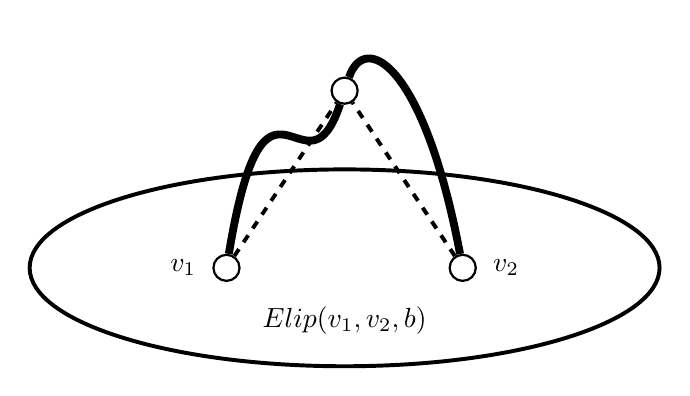
\begin{tikzpicture}[x=1cm, y=0.75cm]
  \begin{scope}[every node/.style={circle,thick,draw}]
\node[label=left:$v_1$](1) at (0,0) {};
\node[label=right:$v_2$](2) at (3,0) {};
\node(3) at (1.5, 3) {};
\end{scope}

\draw[dashed, line width=0.5mm] (1) -- (3);
\draw[dashed, line width=0.5mm] (2) -- (3);
\draw[line width=1mm] (1) .. controls (0.5, 4) and (1, 1) .. (3);
\draw [line width=1mm] (3) .. controls (1.75, 4) and (2.5, 3.5) .. (2);

\draw[line width=0.5mm] (1.5, 0) ellipse (4 cm and 1.25cm) node [below=10pt] {$Elip(v_1, v_2, b)$};
\end{tikzpicture}
\end{center}
\caption{Illustration of \citeauthor{lu2015arc}'s ellipse pruning technique. The goal is to connect $v_1$ to $v_2$ with a path of budget $b$. The bold path is excluded from the search since it contains a point outside of the ellipse \cite{lu2015arc}.}
\label{fig:ellipse}
\end{figure}






\subsection{GraphHopper ILS Implementation}
In my research this term, I decided to implement an ILS algorithm and run it on a real road network using readily available mapping data. The crowd-sourced open mapping dataset \emph{OpenStreetMap} (OSM) was the natural choice for the data. As an organization, OSM  provides a free mapping dataset for the entire planet (a full world map is around 56GB!) \cite{osm}. However, the OSM map format is an XML-based schema which is not trivially translatable into a road network graph. Luckily, in addition to open data, OSM includes a collection of open source software that can interface with the data. Because the goal of this research is not to translate raw OSM data into a usable graph representation, I needed software that already had this parsing capability in order to implement an ILS algorithm.

Because I didn't want to start from scratch, I chose GraphHopper as the starting point for my research. GraphHopper is an open source routing engine written in Java which can download and parse raw OSM data into a usable graph representation \cite{graphhopper}. On top of data parsing, GraphHopper provides a web server and webpage front-end which are useful for visualizing and running routing algorithms. Internally, GraphHopper has a number of built-in pathfinding algorithms including A* and Dijkstra which can be used for routing. These algorithm implementations provide a good template for implementing other routing algorithms with GraphHopper. Additionally, GraphHopper supports multiple ``routing profiles" which modify the weights of roads based on the particular vehicle (e.g. car, bike, walking). 

Because of its simplicity, I chose to implement the VVA algorithm using the GraphHopper engine. Instead of computing all-pairs shortest paths upfront as Algorithm \ref{alg:ils-ver} presupposes, I relied on GraphHopper's built in preprocessing. When running the GraphHopper server for the first time, the engine processes the raw OSM data into a graph and builds contraction hierarchies for each of the enabled routing profiles. Similar to precomputing shortest paths, the method of contraction hierarchies is a preprocessing technique used to speed up shortest-path computations. It works by precomputing ``contracted" versions of the graph that contain shortcuts which means faster traversal later \cite{geisberger2008contraction}. While calculating shortest paths with contraction hierarchies is not as fast as having all paths precomputed, it requires a lot less computation up front. For ease of implementation, I chose to leverage GraphHopper's built in contraction hierarchies to do my arc feasibility checking so I didn not have to write my own preprocessing code. However, using contraction hierarchies does increase implementation complexity a little bit. When running a ``normal" graph traversal algorithm, it is important to ignore the contracted shortcut edges.

\FloatBarrier
\bibliographystyle{plainnat}
\bibliography{references}

\end{document}
